%%%%%%%%%%%%%%%%%%%%%%%%%%%%%%%%%%%%%
% Inlucudings:                      %
%%%%%%%%%%%%%%%%%%%%%%%%%%%%%%%%%{{{%
\documentclass[11pt,english,a4paper,chapterprefix]{scrartcl}
%\usepackage[T1]{fontenc}
\usepackage[bigcaptions]{listing}
%\usepackage[latin1]{inputenc}
\usepackage[small,bf,hang]{caption}
\usepackage[english]{babel}
%\usepackage{epsfig}
\usepackage{wrapfig}
%\usepackage{caption}
\usepackage{psfrag}
\usepackage[rflt]{floatflt}
\usepackage[usenames]{color}
\usepackage{graphicx}
\emergencystretch = 10pt
\usepackage{amsmath}
\usepackage{amssymb}
\usepackage{setspace}
%\usepackage{calc}
\usepackage{tocloft}
\usepackage{listing}
\usepackage{listings}
\usepackage{trsym}
\usepackage{trfsigns}
%\usepackage{minted}
\usepackage{multirow}
\usepackage{fancyhdr}
\usepackage{nomencl}
\usepackage{todonotes}
%\usepackage{float}
\usepackage{subfig}
\usepackage{url}
\usepackage{hyperref}
%\usepackage{listings}
%\input{subsections.sty}
\setcounter{secnumdepth}{5}
\setcounter{tocdepth}{5} 
\numberwithin{equation}{section}
\numberwithin{figure}{section}

% -------------------------------------------
%% glossaries package for list of abbreviations and list of symbols
\usepackage{datatool} % package needed by glossaries
\usepackage[acronym]{glossaries} % *after* hyperref
\newglossary[symlog]{symbol}{symi}{symo}{Symbols}
\makeglossaries
\glstoctrue
\loadglsentries[\acronymtype]{Abbreviations/abbreviations}  % TODO: CAREFUL HERE!!
% -------------------------------------------


%%%%%%%%%%%%%%%%%%%%%%%%%%%%%%%%%}}}%
% New Commands and Configurations:  %
%%%%%%%%%%%%%%%%%%%%%%%%%%%%%%%%%{{{%
%\setkomafont{section}{\Large\rmfamily}
%\setkomafont{subsection}{\large\rmfamily}
%\setkomafont{subsubsection}{\normalsize\rmfamily}
\setkomafont{paragraph}{\footnotesize}
\numberwithin{table}{section}
\numberwithin{listing}{section}
\setlength\textheight{24cm}
\definecolor{orange}{rgb}{1 , 0.5 , 0}
\definecolor{blue}{rgb}{0, 0 , 1}
\definecolor{green}{rgb}{0, 1 ,0}
\newcommand{\cb}{\textcolor{blue}}
\newcommand{\subsubsubsection}{\paragraph}
\newcommand{\subsubsubsubsection}{\subparagraph}
\clubpenalty = 10000
\widowpenalty = 10000
\displaywidowpenalty = 10000
\parindent0pt % No Indent
\makenomenclature
% Document Head
\begin{document}
%\restylefloat{figure}
\pagestyle{fancy}
\rhead{} 

\definecolor{light-gray}{gray}{0.90}

%\lstset{ %
%language=C,                % choose the language of the code
%basicstyle=\small\ttfamily
%,       % the size of the fonts that are used for the code
%%numbers=left,                   % where to put the line-numbers
%numberstyle=\footnotesize,      % the size of the fonts that are used for the line-numbers
%stepnumber=2,                   % the step between two line-numbers. If it's 1 each line 
%                                % will be numbered
%numbersep=5pt,                  % how far the line-numbers are from the code
%backgroundcolor=\color{light-gray},  % choose the background color. You must add \usepackage{color}
%showspaces=false,               % show spaces adding particular underscores
%showstringspaces=false,         % underline spaces within strings
%showtabs=false,                 % show tabs within strings adding particular underscores
%frame=single,                   % adds a frame around the code
%rulecolor= \color{light-gray},
%tabsize=2,                      % sets default tabsize to 2 spaces
%captionpos=b,                   % sets the caption-position to bottom
%breaklines=true,                % sets automatic line breaking
%breakatwhitespace=false,        % sets if automatic breaks should only happen at whitespace
%title=\lstname,                 % show the filename of files included with \lstinputlisting;
%                                % also try caption instead of title
%escapeinside={\%*}{*)},         % if you want to add a comment within your code
%xleftmargin=1cm,
%xrightmargin=1cm,
%morekeywords={*,...}            % if you want to add more keywords to the set
%}
%

%\newminted{perl}{linenos, bgcolor=light-gray, fontsize=\scriptsize}
%\newminted{cpp}{bgcolor=light-gray, fontsize=\scriptsize}
%\newminted{tcl}{bgcolor=light-gray, fontsize=\scriptsize}
%\newminted{sh}{bgcolor=light-gray, fontsize=\scriptsize}
%\newminted{basemake}{bgcolor=light-gray, fontsize=\scriptsize}

%%%%%%%%%%%%%%%%%%%%%%%%%%%%%%%%%}}}%
% fancy nomenclautur:
%%%%%%%%%%%%%%%%%%%%%%%%%%%%%%%%%{{{%
%\setlength{\nomlabelwidth}{.20\hsize}
%\renewcommand{\nomlabel}[1]{#1 \dotfill}

%<*sample05>
\def\@@@nomenclature[#1]#2#3{%
 \def\@tempa{#2}\def\@tempb{#3}%
 \protected@write\@nomenclaturefile{}%
  {\string\nomenclatureentry{#1\nom@verb\@tempa @[{\nom@verb\@tempa}]%
    |nompageref{\begingroup\nom@verb\@tempb\protect\nomeqref{\theequation}}}%
    {\thepage}}%
 \endgroup
 \@esphack}
%\def\nompageref#1#2{%
%  \if@printpageref\pagedeclaration{#2}\else\null\fi
%  \linebreak#1\nomentryend\endgroup}
\def\pagedeclaration#1{\dotfill\nobreakspace ~#1}
%\def\nomentryend{.}
\def\nomlabel#1{\textbf{#1}\hfil}
\makeatletter 
\renewcommand*\dotfill{\leavevmode% 
  \leaders\hbox{$\m@th 
  \mkern \@dotsep mu\hbox{.}\mkern \@dotsep 
  mu$}\hfill\kern\z@} 
\makeatother
%%%%%%%%%%%%%%%%%%%%%%%%%%%%%%%%%}}}%
% Abbr Commands!
%%%%%%%%%%%%%%%%%%%%%%%%%%%%%%%%%{{{%
% \newcommand{\abbr}[2]{\textit{#2} (#1)\nomenclature{#1}{#2 \nomrefpage}}
% \newcommand{\shortabbr}[2]{\nomenclature{#1}{#2 \nomrefpage}}
% \newcommand{\revabbr}[2]{#1 (\textit{#2})\nomenclature{#1}{#2 \nomrefpage}}


%%%%%%%%%%%%%%%%%%%%%%%%%%%%%%%%%}}}%
% Titlepage                         %
%%%%%%%%%%%%%%%%%%%%%%%%%%%%%%%%%{{{%
%%%%%%%%%%%%%%%%%%%%%%%%%%%%%%%%%%%%%%%%%%%%%%%%%%%%%%%%%%%%%%%%%%%%%%%%%%%%%%%%%%%%%%%%%%%%%%%%%%%
\begin{titlepage}
\setcounter{page}{-3}
\begin{center}
\includegraphics*[scale=2.5]{img/TUKL_LOGO.pdf}\\[3ex]

\textsc{\Large University of Kaiserslautern}\\[1.5ex]
Department of Electrical Engineering and Information Technology\\[1.5ex]
Microelectronic Systems Design Research Group \\[3ex]

\vfill
\vfill

\textsc{\Huge Bachelor Thesis}\\[6ex]
\centerline{\Large Design and Implementation of a Blockchain-Based Smart Outlet Concept}
\vspace{20pt}
\centerline{\Large Entwurf und Implementierung eines Blockchain-basierten Smart Outlet Konzepts}

\vfill
\vfill

 \begin{tabular}{rl}\hline\\
 Presented:                & \quad \today \\[1.5ex]
 Author:                   & \quad Daniel Gretzke (392488) \\[1.5ex]
 Research Group Chief:     & \quad Prof.\,Dr.-Ing.\,~N.~Wehn\\[1.5ex]
 Tutor:                    & \quad M.Sc. Frederik Lauer\\[1.5ex]\\\hline
 \end{tabular}
\end{center}

    \clearpage
    \pagestyle{empty}
    \begin{flushleft}
    \section*{Statement}
    \vspace{10mm}
    I declare that this thesis was written solely by myself and exclusively with
    help of the cited resources.

    \vspace{12pt}
    Kaiserslautern, \today \\
%    Kaiserslautern, XXst XXXXXX 2010 \\
    \vspace{20mm}
    Daniel Gretzke
    \end{flushleft}

\end{titlepage}


\newpage

%\clearpage{\pagestyle{empty}\cleardoublepage}
\newpage
% !TEX root = ../diss.tex

\begin{abstract}
\thispagestyle{empty}

\section*{Abstract}

\textcolor{red}{Abstract English here.}

\end{abstract}

%\clearpage{\pagestyle{empty}\cleardoublepage}
\newpage
% !TEX root = ../diss.tex

\begin{abstract}
\thispagestyle{empty}

\section*{Zusammenfassung}

\textcolor{red}{Abstract Deutsch here.}

\end{abstract}

\newpage
%%%%%%%%%%%%%%%%%%%%%%%%%%%%%%%%%}}}%
% Table of Contents                 %
%%%%%%%%%%%%%%%%%%%%%%%%%%%%%%%%%{{{%
\tableofcontents
\newpage
\setcounter{page}{1}
\newpage
%%%%%%%%%%%%%%%%%%%%%%%%%%%%%%%%%}}}%
% Chapters                          %
%%%%%%%%%%%%%%%%%%%%%%%%%%%%%%%%%{{{%
%\onehalfspacing % Stelle 1.5er Abstand ein
%\setstretch{1.1} 
\section{Introduction}
\begin{quote}
  Whereas most technologies tend to automate workers on the periphery doing menial tasks, blockchains automate away the center. Instead of putting the taxi driver out of a job, blockchain puts Uber out of a job and lets the taxi drivers work with the customer directly.
  \\
  {\textit{— Vitalik Buterin, co-founder of Ethereum}}
\end{quote}

A cryptocurrency based on a blockchain was first implemented in 2009 by Satoshi Nakamoto (pseudonym) and was called Bitcoin.
Since then, it has steadily gained importance every year.
Meanwhile, thousands of cryptocurrencies and tokens were built on this technology.
The hype in the year 2017 called the attention of many companies to blockchain and even last year, when the value of cryptocurrencies fell as far as 95\%, the interest in this field did not drop.
\\\\
Compared to traditional payment methods like Visa, Banks and PayPal, cryptocurrencies are built decentralized, meaning that there is no central organization that controls transactions, the issuance of new money, et cetera.
The validity of the blockchain \abbr{peer to peer}{P2P} network is secured through cryptographic protocols.
This brings several benefits.
Traditional payment methods usually go with high transactions costs, most commonly in the amount of a few percent.
On the contrary, the cost of a single transaction on a blockchain averages out at just a few cents\cite{ethereum-fee}.
Some cryptocurrencies even work without any fees.
\\\\
Because of this, they are suited for micro transactions really well.
There are some disadvantages, though.
The blockchain technology is still at an early stage and really immature.
Compared to traditional electronic payments, it only manages to achieve very few \abbr{transactions per second}{TPS} and has long transaction times.
E.g., Bitcoin manages 4-5 TPS\cite{bitcoinTPS} as opposed to Visa, which manages to process almost 4,000 TPS on average\cite{visa}.
\\\\
As stated in the quote above, the key strength of blockchain and cryptocurrencies is the decentralization aspect.
For many, it will reshape various markets we know today, potentially revolutionize the financial industry and even disrupt monopolies in the future.
\\\\
Another trend regarding the future are electric cars.
It's expected that in a few years most cars on the road and almost all cars sold will be electric.
Often these need to be charged overnight.
Unfortunately, most city residents are familiar with the problem that they rarely park in front of their own house, let alone own a garage.
It's foreseeable that recharging your car might bring difficulties.
\\\\ 
This bachelor thesis is devoted to this problem.
It examines whether a smart electrical socket, which is placed outside the house by a homeowner, can be used to efficiently sell electricity and which payment method is suited best for this task.
Based on an initial concept, a prototype is to be developed that implements the previously worked out features.
It will serve as an example on how to implement \abbr{machine to machine}{M2M} payments on a microcontroller level.
\newpage
\clearpage
%\input{2.usw.usw}
%\newpage
%\clearpage
%%%%%%%%%%%%%%%%%%%%%%%%%%%%%%%%%}}}%
% Appendix                          %
%%%%%%%%%%%%%%%%%%%%%%%%%%%%%%%%%{{{%
\newpage
\clearpage

%clear headers
\fancyhead{}
\fancyfoot{}
\fancyfoot[CO, CE] {\thepage}

%\section{Appendix}

%%%%%%%%%%%%%%%% >INSERT YOUR APPENDIX HERE>
\section{Appendix}
\label{sec:appendix}
\subsection{Setup Instructions}
This section will focus on the technical setup of the hardware components of a functioning prototype and the installation and setup of all required software.
\\
\subsubsection{Socket}
The Sonoff S20 smart socket was used for the technical implementation of the concept.
A microcontroller is automatically powered by the socket it is plugged into.
The S20 also has a WiFi module and a relay, which can be switched on and off by the microcontroller.
The microcontroller can be reprogrammed via a serial port.
To program the Sonoff S20 the device has to be opened, revealing the logic board with the relay and the serial port.
\\
\begin{figure}[H]
    \includegraphics[width=\textwidth]{img/S20_open.png}
    \caption{Sonoff S20}
    \label{fig:S20}
\end{figure}
\newpage
To program the microcontroller with a computer a FTDI USB to serial converter is used.
The converter has to be plugged into the S20 as follows:
\\
\begin{center}
    \begin{tabular} { |c|c| }
        \hline
        FTDI Converter & Sonoff S20 \\
        \hline\hline
        GND & GND \\
        \hline
        TX & RX \\
        \hline
        RX & TX \\
        \hline
        3.3V & 3.3V \\
        \hline
    \end{tabular}
    \captionof{table}{Connection between serial converter and microcontroller pins}
    \label{tab:ftdi}
\end{center}
\leavevmode
\\
It's important to notice that the FTDI converter must operate at 3.3V entirely.
Caution: some converters only switch the TX and RX pin to 3.3V while the VCC remains at 5V.
This can fry the internals of the S20.
To program the microcontroller, the button has to be pressed before plugging the pins into the serial port to put it in programming mode.
After the pins have been inserted, the button can be released shortly after.
\\
\begin{figure}[H]
    \includegraphics[width=\textwidth]{img/serial_port.png}
    \caption{Serial ports of the Sonoff S20}
    \label{fig:S20_serial}
\end{figure}
\newpage
Both, the socket and the plug, are programmed using the Arduino IDE.
The following steps need to be followed to install the ESP8266 Board, which the S20 is based on:

\begin{itemize}
    \item Inside the Arduino IDE open "Preferences"
    \item Enter \url{http://arduino.esp8266.com/stable/package_esp8266com_index.json} under "Additional Boards Manager URLs"
    \item Open Tools $\rightarrow$ Board $\rightarrow$ Boards Manager
    \item Search and install "esp8266" by "ESP8266 Community"
\end{itemize}

After connecting the FTDI converter to the computer, it should appear under Tools $\rightarrow$ Port.
To successfully flash code to the S20 the following settings have to be set:

\begin{itemize}
    \item \textit{Board}: "Generic ESP8266 Module"
    \item \textit{CPU Frequency}: "80 MHz"
    \item \textit{Flash Size}: "1M (no SPIFFS)"
\end{itemize}
\leavevmode
\subsubsection{Plug}
The device to control the measurement of current in the plug and handle the communication with the socket is the Heltec WiFi Kit 8, which is based on an ESP8266 as well and has a 0.91 inch OLED display.
\\
\begin{figure}[H]
    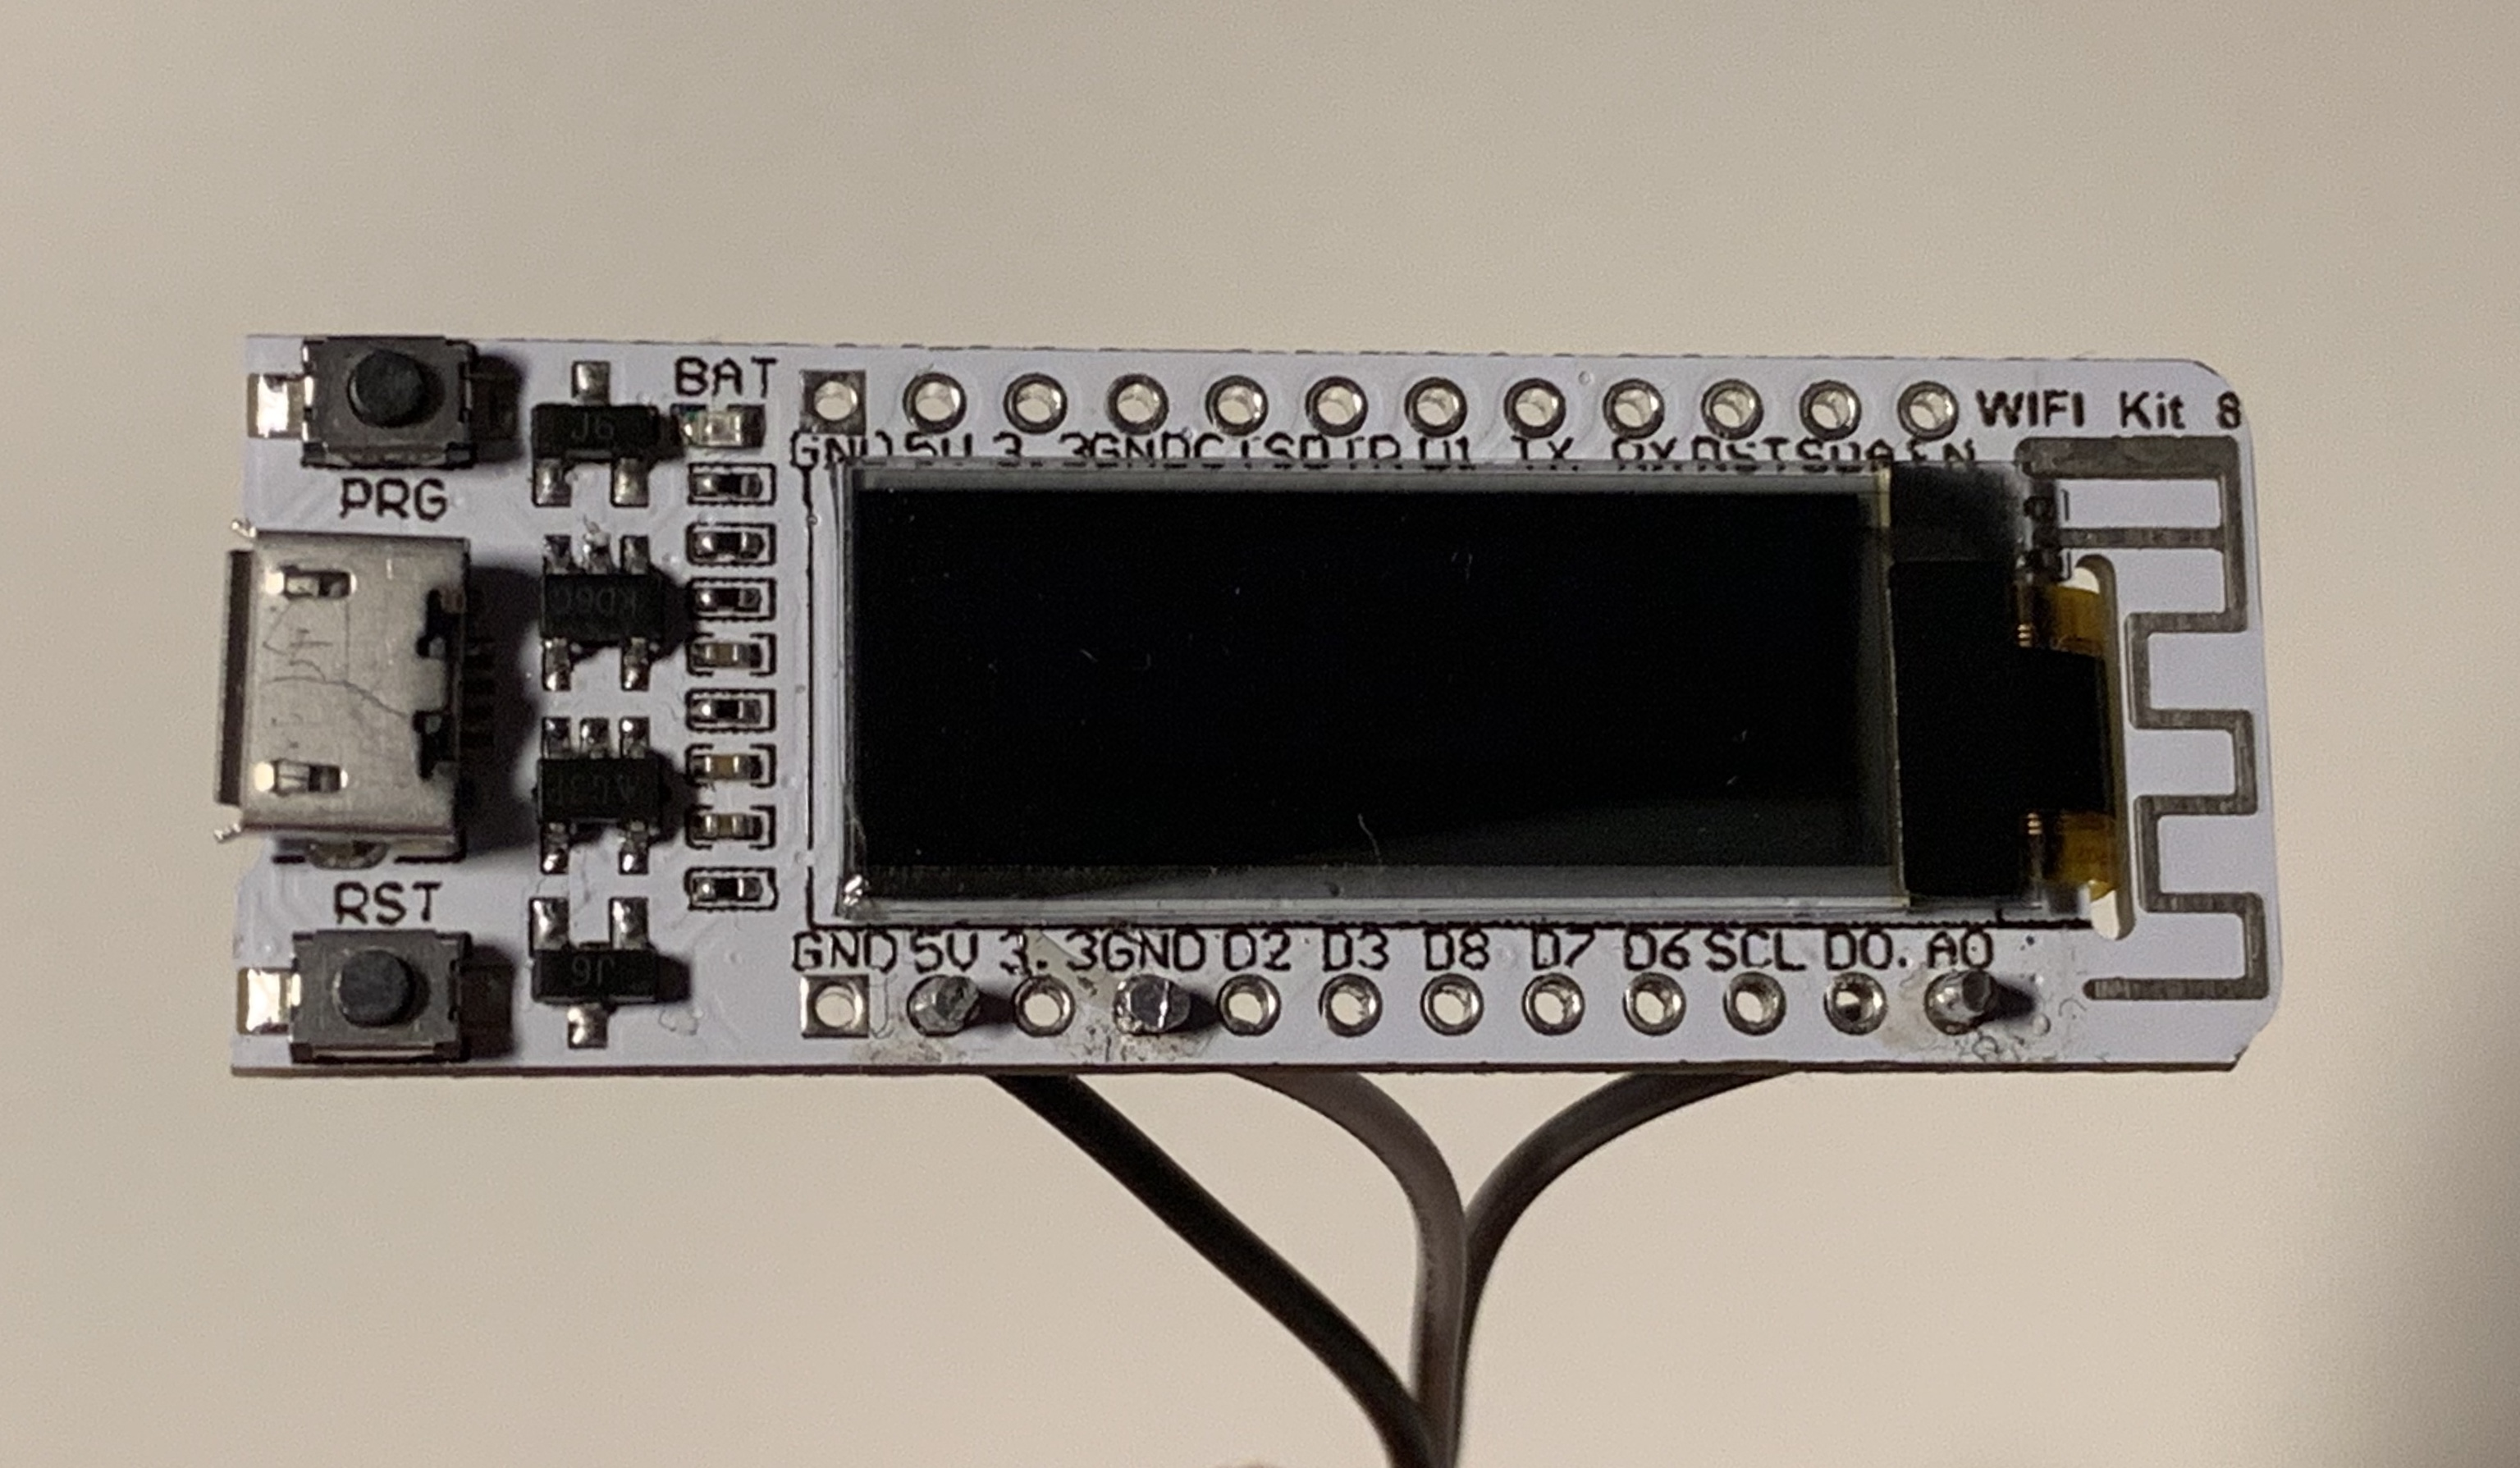
\includegraphics[width=\textwidth]{img/heltec.jpg}
    \caption{Heltec WiFi Kit 8}
    \label{fig:heltec}
\end{figure}

The ACS712 20A current meter is used to measure the current.
It's hall effect-based and provides galvanic isolation up to a minimum of 2.1 kV (RMS)\cite{acs712}.
To connect the current meter, a part of the hot wire leading to the plug has to be cut and stripped.
Both ends have to be inserted into the screw terminal of the ACS712.
The current from the plug is now redirected underneath the hall sensor.
\\
\begin{figure}[H]
    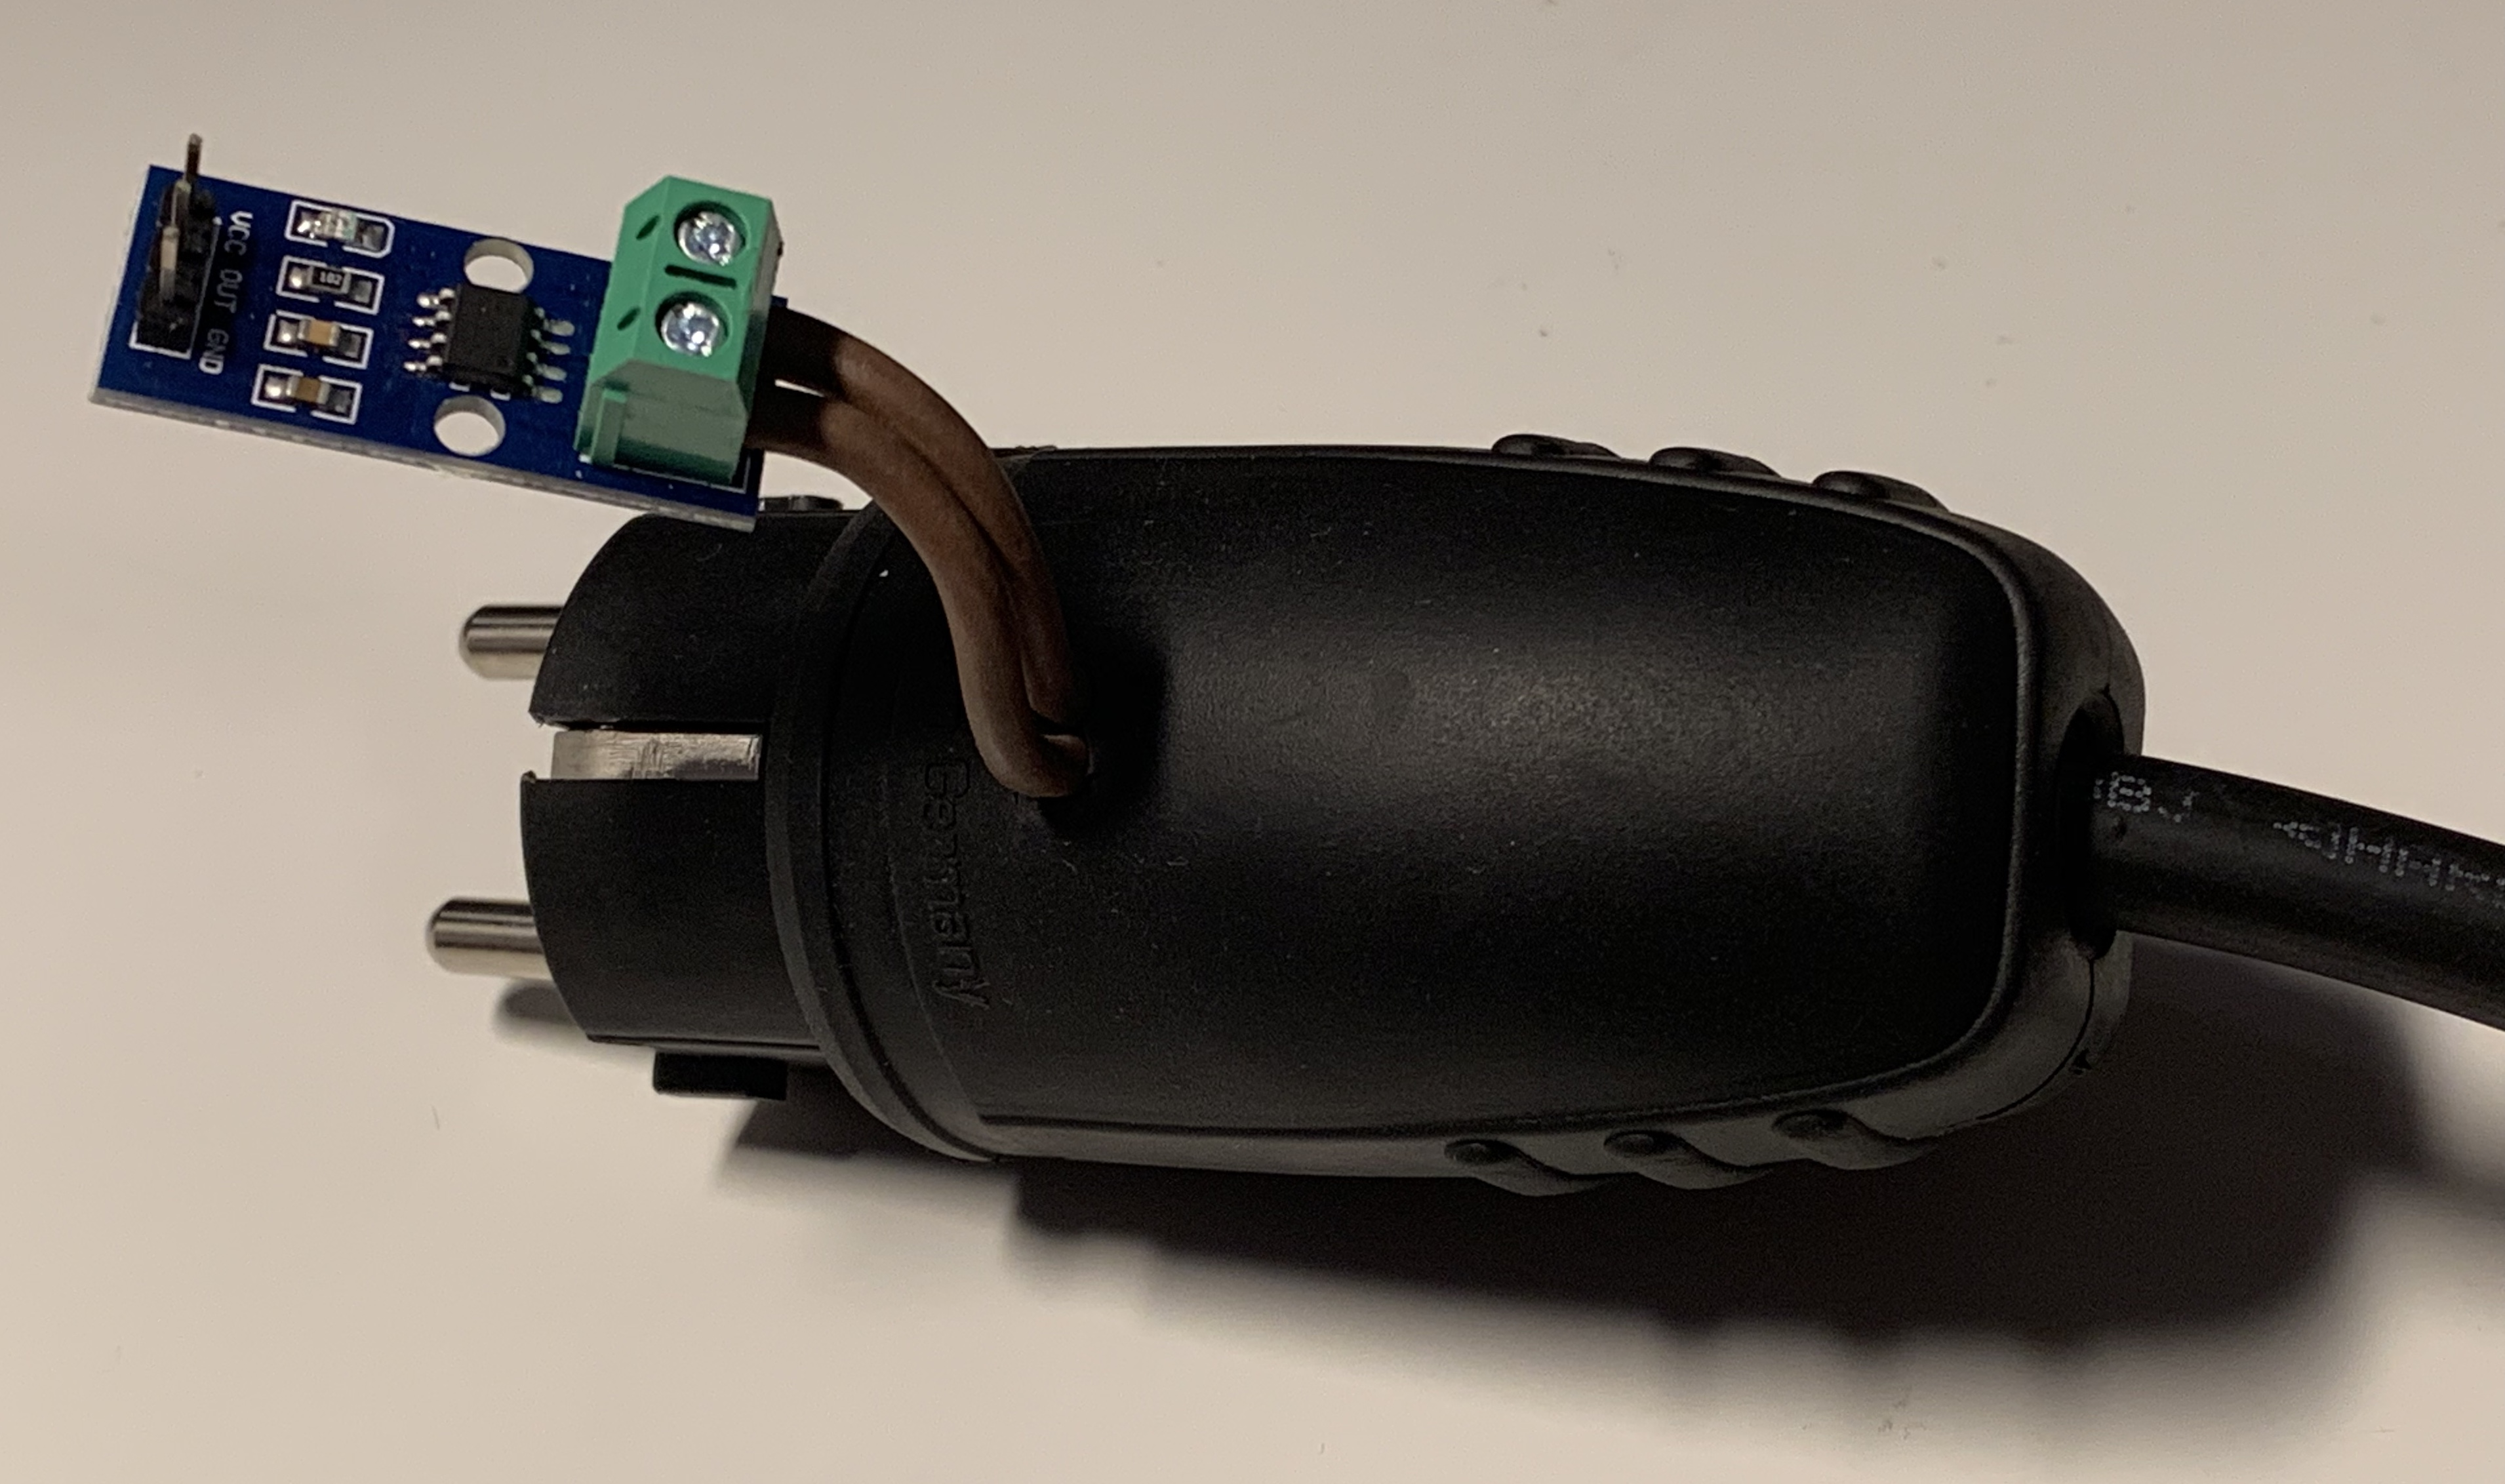
\includegraphics[width=\textwidth]{img/acs712.jpg}
    \caption{ACS712 current meter connected to plug}
    \label{fig:acs712}
\end{figure}

The pins of the current meter have to be soldered to the Heltec board as follows:
\\
\begin{center}
    \begin{tabular} { |c|c| }
        \hline
        ACS712 & Heltec WiFi Kit 8 \\
        \hline\hline
        VCC & 5V \\
        \hline
        OUT & A0 \\
        \hline
        GND & GND \\
        \hline
    \end{tabular}
    \captionof{table}{Connection between current meter and microcontroller pins}
    \label{tab:currentmeter}
\end{center}
\leavevmode
\\
To program the Heltec WiFi Kit 8, USB to UART drivers need to be installed first.
The download link can be found under "References"\cite{vcp-drivers}.
Next, if the ESP8266 was not installed inside the Arduino IDE yet, the instructions found in the subsection above can be used to install the board.
\\
After a successful driver installation, the board should be found under Tools $\rightarrow$ Port when the device is connected to the computer.
\newpage
The following settings are required to ensure a successful flash of the Heltec WiFi Kit:

\begin{itemize}
    \item \textit{Board}: "NodeMCU 1.0 (ESP-12E Module)"
    \item \textit{CPU Frequency}: "160 MHz"
    \item \textit{Flash Size}: "4M (3M SPIFFS)"
\end{itemize}
\leavevmode
\subsubsection{Libraries}
The prototype relies on some external libraries that have to be installed additionally:
\\\\
\textbf{Display}\\
To use the display of the Heltec WiFi Kit a special library needs to be installed.
Inside the Arduino IDE, under Sketch $\rightarrow$ Include Library $\rightarrow$ Manage Library search for and install the "U8g2" library by "oliver".
\\\\
\textbf{WebSocket server}\\
The communication between the plug and the socket relies on WebSockets.
Download the library as a zip file from the git repository\cite{websockets}.
\\
Install it via Sketch $\rightarrow$ Include Library $\rightarrow$ Add .ZIP Library.
\\\\
\textbf{Keccak-256 Library}\\
The implementation relies on a library that was written by Aleksey Kravchenko and was found in the source code of the firefly DIY hardware wallet\cite{keccak-source}.
This library is included with the source code.
\\\\
\textbf{ECDSA Library}\\
Ethereum relies on the Elliptic Curve Digital Signature Algorithm, although there are some differences to the standard implementation of that algorithm.
The zip library is provided with the source code of this prototype and extends the "micro-ecc" library by Kenneth MacKay\cite{micro-ecc}.
\\
\subsubsection{Node}
A server is mandatory to act as a gateway to the Ethereum blockchain.
Geth is the official "Golang implementation of the Ethereum protocol"\cite{geth} and is used to run a full node.
After the installation it will be used to send transactions and make smart contract calls.
\\\\
A \abbr{Virtual Private Server}{VPS} was used for this implementation running Ubuntu 18.04. The server has a six core CPU, 16 GB of RAM, 400GB SSD and 400 MBit/s unlimited traffic.
The following instructions can be used to install the program under Ubuntu.
For other environments the link to the instructions can be found under "References"\cite{geth-instructions}.
To install geth add the repository first:
\begin{lstlisting}[language=bash, numbers=none]
  $ sudo add-apt-repository -y ppa:ethereum/ethereum
\end{lstlisting}

Next, install geth:
\begin{lstlisting}[language=bash, numbers=none]
  $ sudo apt-get update
  $ sudo apt-get install ethereum
\end{lstlisting}
\leavevmode
\\
To interact with the Ethereum blockchain the entire chain history has to be downloaded first.
This can take up to 40 GB of disk space and will take several hours of synchronizing.
Geth will be started via this console command:
\begin{lstlisting}[language=bash, showstringspaces=false, numbers=none]
  $ geth console --rinkeby --rpc --rpcapi="db,eth,net,web3,
  personal,txpool" --rpcaddr X.X.X.X --rpcport 8545 --cache=2048
\end{lstlisting}

The launch options have the following purposes\cite{cli-options}:
\begin{itemize}
    \item \textit{rinkeby}: synchronizes the Rinkeby testnet
    \item \textit{rpc}: enables the HTTP-RPC server, allows to receive JSON RPC requests
    \item \textit{rpcapi}: exposed APIs, a listing of all APIs can be found under "References"\cite{json-rpc}\cite{management-apis}
    \item \textit{rpcaddr}: IP address of RPC interface, replace "X.X.X.X" with the IP address of the server, defaults to "localhost".
    Exposing the RPC interface without any restrictions is not advisable, especially on the mainnet, as it is a severe security concern.
    \item \textit{rpcport}: listening port of the RPC server
    \item \textit{cache}: memory allocated in MB, a minimum of 1024 MB is advisable for a faster synchronization
\end{itemize}
The console parameter starts a JavaScript console, allowing to interact with the blockchain using the web3 library.
Geth currently comes with web3 version 0.20.1\cite{javascript-0.20} but might be upgraded to version 1.0\cite{javascript-1.0} soon.
The links to the documentation of both versions can be found under "References".
\\
The version of the web3 library can be checked using:

\begin{lstlisting}[language=bash, numbers=none]
  > web3.version
\end{lstlisting}

The output of the synchronization could hamper the ability to properly read the output of the JavaScript console.
The verbosity can be set via the following command:

\begin{lstlisting}[language=bash, numbers=none]
  > debug.verbosity(x)
\end{lstlisting}

Replace x with 0 for silent, 1 for error, 2 for warn, 3 for info, 4 for debug and 5 for detail.
The verbosity defaults to info\cite{cli-options}.
\newpage

\begin{lstlisting}[language=bash, numbers=none]
  > eth.blockNumber
\end{lstlisting}

returns the block number of the latest synchronized block, which is the amount of all previous blocks.
The first block, the also called the genesis block, starts with the block number 0.
The current block number can be checked through so-called block explorers, e.g., {rinkeby.etherscan.io}.
\\
\begin{lstlisting}[language=bash, numbers=none]
  > eth.syncing
\end{lstlisting}
returns the current block number and the highest block number.
As soon as the client is synchronized it returns "false"\cite{javascript-0.20}.
\\\\
As previously mentioned, the node was set up to accept and handle api calls in the form of http requests, which follow the JSON-RPC 2.0 specification\cite{json-rpc-spec}.
The implementation heavily relies on the API, as it is used to not only fetch data from the blockchain, but also to send transactions and make smart contract calls\cite{json-rpc}\cite{management-apis}.
\\\\
\subsection{Smart Contract}
The following subsections will describe every step of deploying a smart contract to the Rinkeby Ethereum testnet.
\\ 
\subsubsection{Wallet}
The first thing needed to start programming smart contracts is an Ethereum wallet.
MetaMask is a browser extension for Chrome, Firefox and Opera, that not only allows to manage multiple accounts on multiple test chains, it also injects the web3.js library into websites allowing to interact with the Ethereum blockchain and smart contracts on web pages.
Visit the MetaMask\cite{metamask} website and download the browser extension.
A new account will be generated using a mnemonic phrase, defined in the BIP39 (Bitcoin improvement proposal)\cite{bip39}.
It usually consists of 12 words which represent a private key, essentially creating an easy way to remember / write down private keys.
An example for a mnemonic phrase is:
\begin{lstlisting}[language=bash, numbers=none]
  short heavy hidden anger nephew tragic fade dad renew finger among tiny
\end{lstlisting}
This phrase translates to the following seed:
\begin{lstlisting}[language=bash, numbers=none]
  b7b36d9ca1e105045344ecb7ca7b9449bfc0889139c9719876d03cf7b5814861
  37e905b9e94e50c03ca22871937ae3c754dea1427eede8198c6774d90fc1a1f4
\end{lstlisting}

Using the BIP44\cite{bip44} standard an unlimited amount of private keys can be derived from the seed.
For example the first private key derived from this seed would be:
\begin{lstlisting}[language=bash, numbers=none]
  0xfb8502c03ea336344dc44b66b1a3c01e2917138e92bfa93c54725166394cd46b
\end{lstlisting}
with the corresponding address
\begin{lstlisting}[language=bash, numbers=none]
  0x4d43c1E254a9333fB0D8A50BD3f01b6787ee8895
\end{lstlisting}
The second derived private key is:
\begin{lstlisting}[language=bash, numbers=none]
  0x64b45c024041178aff2f9ed7b7026fff6890c871818c39c1c7bd826e6aa33773
\end{lstlisting}
with the corresponding address
\begin{lstlisting}[language=bash, numbers=none]
  0xd38F7dc2d9B6F6D9d5CB6C8813e213D5DC541458
\end{lstlisting}
and so on.
This means that the single mnemonic phrase will act as a backup phrase for all accounts that will be created inside the MetaMask wallet.
After MetaMask was set up create a second account and set the network to Rinkeby.
Ethers are required to send transactions on the testnet and can be received via the website faucet.rinkeby.io.
\\
\subsubsection{IDE}
The smart contract was developed using Remix.
It's an online IDE including a compiler for the languages Solidity and Vyper, various debugging and testing tools and can be found under remix.ethereum.org.
\\
After choosing \textit{Solidity} as an environment a compiler has to be set.
Because the programming language was designed especially for Ethereum, it is still under very heavy development with frequent updates coming out.
The documentation for each specific version can be found under
\\
\url{https://solidity.readthedocs.io/en/v0.5.8/}
\\
while replacing "0.5.8" (the latest stable version at the time of writing) with the desired compiler version.
\\\\
Inside the "Run" tab the connection to the blockchain can be chosen under "Environment".
The most important options are:
\begin{itemize}
    \item \textit{JavaScript VM}: A personal Ethereum blockchain implemented in JavaScript that runs locally.
    It comes with 5 accounts which are preloaded with 100 ETH.
    It's suited for early development stages, unit testing, and all in all quick tests, as there are no transaction times.
    \item \textit{Injected Web3}: As mentioned before, MetaMask injects Web3 into websites.
    When choosing this option, the currently active account and the chosen network in MetaMask are used for development.
\end{itemize}
Underneath, the smart contract can be chosen and deployed to the blockchain.
Next to the deploy button, constructor arguments can be passed.
Optionally an existing smart contract can be loaded from an address.
\\\\
After a contract has been deployed or loaded, all functions and public variables will be listed under the "Deployed Contracts" section.
This will be the main way to interact with the smart contract.
\\\\
\subsubsection{Solidity}
This subsection will explain the basics and key features of the Solidity programming language.
A solidity source file has the ".sol" file extension.
The language has a C++ style syntax and works very similarly to object-oriented programming and is also called contract-oriented\cite{doc-oriented}.
Contracts can be viewed as classes and also work with interfaces and inheritance.
\\
See Listing \ref{lis:sc_basic_ref} for an example of a minimalistic smart contract, which demonstrates the general syntax as well as some of the features listed below.
\\\\
\textbf{General notice}\\
There are a few important aspects in how certain things behave during smart contract programming and execution:
\begin{itemize}
  \item Solidity does not implement floats at the time of writing.
  This is especially important for calculations using Ether.
  Therefore it is important to remember that Ether is always assumed as Wei by smart contract functions.
  \item When a function throws, all changes to the state that were made up to this point are reverted and the transaction is marked as failed.
  \item \textit{undefined} and \textit{null} does not exist in Solidity, variables rather have a default type, e.g., 0 for integers\cite{doc-types}.
\end{itemize}
\leavevmode
\\
\textbf{Types}\\
The most important data types in Solidity are\cite{doc-types}:
\begin{itemize}
  \item \textit{bool}: The possible values are "true" and "false".
  \item \textit{integer}: There are signed (\textit{int}) and unsigned (\textit{uint}) integers in Solidity.
  \textit{uint} is an alias for \textit{uint256}.
  The smallest size for an integer is 8 bit (e.g., \textit{uint8}), the sizes grow by 8 up to 256 bit.
  The same applies to signed integers as well.
  \item \textit{address}: The address variable stores 20 bytes.
  \item \textit{address payable}: The address payable variable stores 20 bytes as well.
  Additionally it holds the members \textit{transfer} and \textit{send} to send Ether to that address.
  \item \textit{bytes32}: Holds 32 bytes of data.
  \item \textit{mapping(keyType $=>$ valueType)}: Mappings work similarly to hash tables.
  The key can be of any elementary type, the value can be of any type, even another mapping.
  An example for a frequently used mapping would be the balance variable:
  \\
  \textit{mapping(address $=>$ uint256) balances;}
  \\
  Every address points to a uint256 which represents a balance.
  \item \textit{bytes[]}: Dynamically-sized byte array.
  \item \textit{string}: Dynamically-sized UTF-8 encoded string.
\end{itemize}
\leavevmode
\\
\textbf{Pragma}\\
The first line of a solidity file defines the compiler version\cite{doc-pragma}:
\begin{lstlisting}[language=Solidity, numbers=none]
  pragma solidity ^0.5.4;
\end{lstlisting}
The \^{} symbol means that the code can be compiled by a compiler with the versions 0.5.4 and above, but below 0.6.0. Without the \^{} symbol only the compiler version 0.5.4 can compile the source code.
\\\\
\textbf{Important variables and functions}\\
Solidity features some global units, variables and functions which can be very useful, if not necessary for smart contract programming:
\begin{itemize}
  \item \textit{ether}: The ether unit multiplies the current value by \(10^{18}\), e.g., 3 ether equals 3,000,000,000,000,000,000.
  \item \textit{time units}: The following time units are available: "seconds", "minutes", "hours", "days", "weeks".
  1 seconds equals 1, 1 minutes equals 60 seconds or 60, 1 hours equals 60 minutes or 3600 and so on.
  \item \textit{now}: An alias for \textit{block.timestamp}, a \textit{uint256} variable as seconds since unix epoch.
  The variable is set by the miner during validation so it should not be used for random number generation as the number can be varied by up to $\pm$ 15 seconds, because the timestamp of a block has to be higher than the one of the previous block.
  \item \textit{msg.sender}: Of type \textit{address payable} and contains the sender of the current message.
  If a function is called directly by an EOA and not by a smart contract, \textit{msg.sender} will contain the sender of the transaction.
  \item \textit{msg.value}: Of type \textit{uint256} and contains the number of Wei sent with the current message.
  \item \textit{$<$address payable$>$.transfer(uint256 value)/$<$address payable$>$.send(uint256 value)}: Both functions send "value" in Wei to the payable address.
  Transfer throws, send returns false on failure.
  \item \textit{function ()}: A function declared without any name is also called the fallback function.
  This function is called, when no matching function identifier is provided.
  Usually this function is triggered, when a simple transaction is sent to the smart contract, that's why the fallback function can often be seen with the \textit{payable} modifier.
  \item \textit{require(bool condition, string memory message)}: The require function throws if the condition is not met and provides the custom error message.
  \item \textit{keccak256(bytes memory) returns (bytes32)}: Computes the Keccak-256 hash of an input.
  \item \textit{ecrecover(bytes32 hash, uint8 v, bytes32 r, bytes32 s) returns (address)}: For a given message and r, s, v values of a ECDSA signature the function returns the address associated with the public key from the signature.
\end{itemize}
\leavevmode
\\
\textbf{Constructor}\\
A constructor function is optional and can be used to execute code directly when the smart contract is stored on the blockchain\cite{doc-constructor}.
\\\\
\textbf{Modifiers}\\
A function can have multiple different modifiers, that make it behave in different ways\cite{doc-modifiers}.
First, there is the visibility modifier, which manages the access to functions and variables:
\begin{itemize}
  \item \textit{public}: The public modifier makes a function visible from inside and outside the smart contract.
  Adding the modifier to a variable automatically generates a getter function with the same name as the variable.
  \item \textit{external}: The external modifier is only applicable for functions.
  It makes them only visible from outside the smart contract.
  To call the function from inside the smart contract it has to be called via "this.func()" instead of "func()".
  \item \textit{internal}: The internal modifier makes a function or variable only visible internally.
  This means they can only be accessed from the contract and all derived contracts.
  \item \textit{private}: The private modifier makes a function or variable only visible from the contract itself.
  It's important to notice that although a variable might be private, it still can be read, since all data stored on the blockchain is public.
\end{itemize} 
\leavevmode
\\
Reading from the blockchain does not require mining or involve transaction fees.
Therefore functions that do not write to storage can be marked as such via a modifier:
\begin{itemize}
  \item \textit{view}: If a function has a view modifier, it cannot write to storage, only read from it.
  \item \textit{pure}: If a function has a pure modifier, it cannot modify storage.
  Additionally it cannot read state, e.g., read from variables.
  It's primarily used for computations.
\end{itemize}
\leavevmode
\\
The \textit{payable} modifier allows a function to receive Ether.
If Ether is included in a function call that doesn't have the \textit{payable} modifier, it throws.
\\\\
It's also possible to write custom modifiers.
Listing \ref{lis:sc_basic_ref} shows the function of a custom modifier through a commonly used \textit{onlyOwner} modifier, which only allows the owner of a smart contract to call the function.
\\\\
\textbf{Events}\\
Events are an important part of smart contract programming for two key reasons:
\begin{enumerate}
  \item With a complex smart contract handling thousands of transactions, it can get confusing to keep track of all changes made to the state of the smart contract.
  Events are a good way to sort these changes into different categories and make them searchable by specific filters.
  \item Some time passes until a transaction was mined, therefore the return value of a function is not returned to the sender of the transaction.
  Events can be used to act as a return value.
  A computer system or a frontend can then scan for these events and act accordingly, e.g., show updates to the user.
\end{enumerate}
See Listing \ref{lis:sc_basic_ref} for an example of an event.
\\\\
\begin{lstlisting}[language=Solidity, caption={Basic structure of a smart contract}, label={lis:sc_basic_ref}]
pragma solidity 0.5.8;

contract ModifierExample{
    // variable to store the owner of the smart contract
    address owner;
    // number to demonstrate the view function
    uint256 public num;
    
    // definition of an event
    // the indexed keyword allows to use the parameter as a filter
    event ownerChanged(address indexed oldOwner, address indexed newOwner);
    
    // the constructor gets called after contract creation
    // arguments can be passed to the constructor
    constructor(uint256 _num) public {
        // set owner to the sender of the transaction
        owner = msg.sender;
        // set the number to the passed argument
        num = _num;
    }
    
    // custom modifier
    modifier onlyOwner() {
        // throws if sender of call is unequal to value stored in owner variable
        require(owner == msg.sender, "sender is not owner");
        // _; defines where the code of the function, the modifier is used on, runs
        _;
    }
    
    // function to change the address of the smart contract
    function changeOwner(address _owner) external onlyOwner {
        // emits the ownerChanged event
        emit ownerChanged(owner, _owner);
        // sets the owner variable to the passed argument
        owner = _owner;
    }
    
    // the function will execute the code and return the calculated number
    // because of the view modifier no state is modified and no transaction has to be sent
    function calculatedNum() public view returns(uint256) {
        return num * 2;
    }
    
}
\end{lstlisting}
\leavevmode
\\
\textbf{Libraries}\\
Libraries can be used to reduce code redundancy and save transaction fees.
For the implementation of this smart contract, a so-called SafeMath library was used to detect integer over- and underflows.
An example on how to use a library for a certain data type can be found in line 70 of the smart contract source code:
\\
\begin{lstlisting}[language=Solidity, caption={Using the SafeMath library}, label={lis:safemath_use}, firstnumber=70]
using SafeMath for uint256;
\end{lstlisting}
Here are some examples on how to add, subtract or multiply integers using the library.
\\
\begin{lstlisting}[language=Solidity, caption={Examples for SafeMath calculations}, label={lis:safemath_example}]
uint256 a = 5;
uint256 b = 7;

// add two integers
// c = a + b
uint256 c = a.add(b)

// subtract two integers
// d = b - a
// would result in an integer underflow, therefore the safemath library throws
uint256 d = b.sub(a)

// multiply two integers
// e = a * b
uint256 e = a.mul(b)
\end{lstlisting}
\subsubsection{Source Code}


% https://tex.stackexchange.com/questions/264361/skipping-line-numbers-in-lstlisting/264373#264373
\lstset{numbers=left,numberblanklines=true,escapeinside=||}

\let\origthelstnumber\thelstnumber
\makeatletter
\newcommand*\Suppressnumber{%
  \lst@AddToHook{OnNewLine}{%
    \let\thelstnumber\relax%
     \advance\c@lstnumber-\@ne\relax%
    }%
}

\newcommand*\Reactivatenumber[1]{%
  \setcounter{lstnumber}{\numexpr#1-1\relax}
  \lst@AddToHook{OnNewLine}{%
   \let\thelstnumber\origthelstnumber%
   \refstepcounter{lstnumber}
  }%
}

\begin{lstlisting}[language=Solidity, caption={SafeMath library}, label={lis:safemath}, firstnumber=3]
/**
 * @title SafeMath
 * @dev Unsigned math operations with safety checks that revert on error
 * @notice https://github.com/OpenZeppelin/openzeppelin-solidity
 */
library SafeMath {
    /**
     * @dev Multiplies two unsigned integers, reverts on overflow.
     */
    function mul(uint256 a, uint256 b) internal pure returns (uint256) {
        // Gas optimization: this is cheaper than requiring 'a' not being zero, but the
        // benefit is lost if 'b' is also tested.
        // See: https://github.com/OpenZeppelin/openzeppelin-solidity/pull/522
        if (a == 0) {
            return 0;
        }

        uint256 c = a * b;
        require(c / a == b);

        return c;
    }

    /**
     * @dev Integer division of two unsigned integers truncating the quotient, reverts on division by zero.
     */
    function div(uint256 a, uint256 b) internal pure returns (uint256) {
        // Solidity only automatically asserts when dividing by 0
        require(b > 0);
        uint256 c = a / b;
        // assert(a == b * c + a % b); // There is no case in which this doesn't hold

        return c;
    }

    /**
     * @dev Subtracts two unsigned integers, reverts on overflow (i.e. if subtrahend is greater than minuend).
     */
    function sub(uint256 a, uint256 b) internal pure returns (uint256) {
        require(b <= a);
        uint256 c = a - b;

        return c;
    }

    /**
     * @dev Adds two unsigned integers, reverts on overflow.
     */
    function add(uint256 a, uint256 b) internal pure returns (uint256) {
        uint256 c = a + b;
        require(c >= a);

        return c;
    }

    /**
     * @dev Divides two unsigned integers and returns the remainder (unsigned integer modulo),
     * reverts when dividing by zero.
     */
    function mod(uint256 a, uint256 b) internal pure returns (uint256) {
        require(b != 0);
        return a % b;
    }
}
\end{lstlisting}
\begin{lstlisting}[language=Solidity, caption={Payment channel smart contract}, label={lis:pc_sc}]
pragma solidity ^0.5.0;|\Suppressnumber|

library SafeMath {
    // insert SafeMath library code from above
}
|\Reactivatenumber{68}|
contract SocketPaymentChannel {
    // use the SafeMath library for calculations with uint256 to prevent integer over- and underflows
    using SafeMath for uint256;

    address public owner;
    uint256 public pricePerSecond;

    // stores the balances of all customers and the owner
    mapping(address => uint256) public balances;

    // duration after a payment channel expires in seconds
    uint256 public expirationDuration;
    // minimum required deposit for payment channel
    uint256 public minDeposit;

    // global payment channel variables
    // boolean whether the payment channel is currently active
    bool public channelActive;
    // timestamp when payment channel was initialized
    uint256 public creationTimeStamp;
    // timestamp when payment channel will expire
    uint256 public expirationDate;
    // address of current customer
    address public channelCustomer;
    // value deposited into the smart contract
    uint256 public maxValue;

    // nonces to prevent replay attacks
    mapping(address => uint256) public customerNonces;

    // events
    event InitializedPaymentChannel(address indexed customer, uint256 indexed start, uint256 indexed maxValue, uint256 end);
    event ClosedPaymentChannel(address indexed sender, uint256 indexed value, bool indexed expired, uint256 duration);
    event PriceChanged(uint256 indexed oldPrice, uint256 indexed newPrice);
    event Withdrawal(address indexed sender, uint256 indexed amount);

    // modifier that only allows the owner to execute a function
    modifier onlyOwner() {
        require(msg.sender == owner, "sender is not owner");
        _;
    }

    constructor(uint256 _pricePerSecond, uint256 _expirationDuration, uint256 _minDeposit) public {
        owner = msg.sender;
        pricePerSecond = _pricePerSecond;
        expirationDuration = _expirationDuration;
        minDeposit = _minDeposit;
        channelActive = false;
    }

    /// @notice function to initialize a payment channel
    /// @return true on success, false on failure
    function initializePaymentChannel() public payable returns (bool) {
        // payment channel has to be inactive
        require(!channelActive, "payment channel already active");
        // value sent with the transaction has to be at least as much as the minimum required deposit
        require(msg.value >= minDeposit, "minimum deposit value not reached");

        // set global payment channel information
        channelActive = true;
        // set channel customer to the address of the caller of the transaction
        channelCustomer = msg.sender;
        // set the maximum transaction value to the deposited value
        maxValue = msg.value;
        // set the timestamp of the payment channel intialization
        creationTimeStamp = now;
        // calculate and set the expiration timestamp
        expirationDate = now.add(expirationDuration);

        // emit the initialization event
        // It's cheaper in gas to use msg.sender instead of loading the channelCustomer variable, msg.value instead of maxValue, etc.
        emit InitializedPaymentChannel(msg.sender, now, now.add(expirationDuration), msg.value);
        return true;
    }

    /// @notice function to close a payment channel and settle the transaction
    /// @dev can only be called by owner
    /// @param _value the total value of the payment channel
    /// @param _signature the signature of the last off-chain transaction containing the total value
    /// @return true on success, false on failure
    function closeChannel(uint256 _value, bytes memory _signature) public onlyOwner returns (bool) {
        // save value to a temporary variable, as it is reassigned later
        uint256 value = _value;
        // payment channel has to be active
        require(channelActive, "payment channel not active");
        // call verify signature function, if it returns false, the signature is invalid and the function throws
        require(verifySignature(value, _signature), "signature not valid");

        // increase nonce after payment channel is closed
        customerNonces[channelCustomer] = customerNonces[channelCustomer].add(1);

        // if maxValue was exceeded, set value to maxValue
        if (value > maxValue) {
            value = maxValue;
            // value of payment channel equals the exact deposited amount
            // credit owner the total value
            balances[owner] = balances[owner].add(value);
        } else {
            // credit owner the value from the payment channel
            balances[owner] = balances[owner].add(value);
            // refund the remaining value to the customer
            balances[channelCustomer] = balances[channelCustomer].add(maxValue.sub(value));
        }

        // emit payment channel closure event
        emit ClosedPaymentChannel(msg.sender, value, false, now - creationTimeStamp);

        // reset channel information
        channelActive = false;
        channelCustomer = address(0);
        maxValue = 0;
        expirationDate = 0;
        creationTimeStamp = 0;

        return true;
    }

    /// @notice function to timeout a payment channel, refunds entire deposited amount to customer
    /// @return true on success, false on failure
    function timeOutChannel() public returns (bool) {
        // payment channel has to be active
        require(channelActive, "payment channel not active");
        // payment channel has to be expired
        require(now > expirationDate, "payment channel not expired yet");

        // increase nonce after payment channel is closed
        customerNonces[channelCustomer] = customerNonces[channelCustomer].add(1);

        // return funds to customer if channel was not closed before channel expiration date
        balances[channelCustomer] = balances[channelCustomer].add(maxValue);

        // emit payment channel closure event
        emit ClosedPaymentChannel(msg.sender, 0, true, now - creationTimeStamp);

        // reset channel information
        channelActive = false;
        channelCustomer = address(0);
        maxValue = 0;
        expirationDate = 0;
        creationTimeStamp = 0;

        return true;
    }

    /// @notice helper function to validate off-chain transactions
    /// @param _value value of the off-chain transaction
    /// @param _signature signature / off-chain transaction
    /// @return true if the sender of the off-chain transaction is equal to the current customer, else false
    function verifySignature(uint256 _value, bytes memory _signature) public view returns (bool) {

        // split signature into r,s,v values (https://programtheblockchain.com/posts/2018/02/17/signing-and-verifying-messages-in-ethereum/)
        require(_signature.length == 65, "signature length is not 65 bytes");

        bytes32 r;
        bytes32 s;
        uint8 v;

        // split using inline assembly
        assembly {
            // first 32 bytes of message
            r := mload(add(_signature, 32))
            // second 32 bytes of message
            s := mload(add(_signature, 64))
            // first byte of the next 32 bytes
            v := byte(0, mload(add(_signature, 96)))
        }

        // to recover the address of the sender, the signed data has to be recreated
        // variables that are included in the message: value, address of contract, nonce of customer
        address contractAddress = address(this);
        // hash variables
        bytes32 message = keccak256(abi.encodePacked(_value, contractAddress, customerNonces[channelCustomer]));
        // prefix message with ethereum specific prefix
        bytes32 prefixedMessage = keccak256(abi.encodePacked("\x19Ethereum Signed Message:\n32", message));
        // ecrecover recovers the address from a signature and the signed data
        // returns true if recovered address is equal to customer address
        return ecrecover(prefixedMessage, v, r, s) == channelCustomer;
    }

    /// @notice function to withdraw funds from the smart contract
    /// @return true on success, false on failure
    function withdraw() public returns (bool) {
        // save balance of sender to a variable
        uint256 balance = balances[msg.sender];
        // best practice: set balance of sender to zero before sending the transaction, see reentrancy attack
        balances[msg.sender] = 0;
        // send entire balance to sender
        msg.sender.transfer(balance);
        // emit withdrawal event
        emit Withdrawal(msg.sender, balance);
        return true;
    }

    /// @notice function to change the electricity price, only callable by the owner
    function changePrice(uint256 _newPrice) public onlyOwner {
        // emit price changed event
        emit PriceChanged(pricePerSecond, _newPrice);
        // update price per second
        pricePerSecond = _newPrice;
    }
}
\end{lstlisting}
\newpage
\clearpage
%\addcontentsline{toc}{section}{Appendix}
%List of Figures
\vspace{-20pt}
\begingroup
    \addcontentsline{toc}{subsection}{List of Figures}
    \setlength{\cftparskip}{10pt}
    \listoffigures 
\endgroup
\newpage
\clearpage
%List of Tables
\begingroup
    \addcontentsline{toc}{subsection}{List of Tables}
    \setlength{\cftparskip}{10pt}
    \listoftables
\endgroup
\newpage
\clearpage
%List of Listings
%\renewcommand{\lstlistlistingname}{Verzeichnis der Quellcodes}
\begingroup
    \addcontentsline{toc}{subsection}{List of Listings}
      \setlength{\itemsep}{20pt}
  \setlength{\parskip}{10pt}
    \renewcommand{\listlistingname}{List of Listings}
    \listoflistings 
\endgroup
\newpage
\clearpage
%List of Abbreviations
% \begingroup
%     \addcontentsline{toc}{subsection}{List of Abbreviations}
%     \renewcommand{\nomname}{List of Abbreviations}
%     \renewcommand{\nompreamble}{\vspace{10pt}}
%     %\setlength{\nomitemsep}{8pt}
%     \printnomenclature[2cm]
% \endgroup
\newpage
\clearpage
%Literatur:
\addcontentsline{toc}{subsection}{References}
\bibliographystyle{unsrt}
\bibliography{doc}
%%%%%%%%%%%%%%%%%%%%%%%%%%%%%%%%%}}}%
\end{document}
